\documentclass[onecolumn, preprint]{sigplanconf}
\usepackage{multicol}
\usepackage{listings}
\usepackage{comment}
\usepackage{graphicx}

\title{COS 597B: Final Report\\
\emph{Towards SMT in VST}}

\authorinfo{Santiago Cuellar \and Olivier Savary B\'{e}langer}
           {Princeton University}
           {scuellar/olivierb@princeton.edu}

\begin{document}
\maketitle


%start
\section{Introduction}
When formally proving the function correctness of programs, a portion of the proof or lemmas require a level of intuition or higher-order reasoning which goes beyond what is supported by automated theorem prover. However, between these crucial steps are many mechanical ones. Certain interactive theorem provers such as Coq provide scripting facilities to automate these steps, but this limited form of automation is ad hoc and brittle. It has been observed that many of these steps corresponds to reasoning over STM theories which can be performed by existing STM solvers. 

The goal of the project is to investigate using an SMT solver to discharge obligations generated by VST. After investigated the currently available tools to interface Coq and SMT solvers, we found out that SMTCoq already implements a pipeline from Coq goals to SMTLib and back into Coq after being solved by an SMT solver producing evidences. However, limitations in the current versions of SMTcoq, SMTlib and SMT solvers interfacing with SMTlib and SMTcoq prevent us from experimenting this pipeline. Our contributions are
\begin{itemize}
 \item identifing goals in VST development which could be reduce to formulas in SMT theories
 \item identifing the theories needed for such development to be useful
 \item sketching a completed pipeline assuming minimal updates to relevant tools
 \item defining encoding of list-reasoning in the theory of arrays with uninterpreted functions (\emph{QF\_AUFLIA})
 \item proving the soundness of this encoding
\end{itemize}

This report is organized as follow: Section 2 provide backgrounds about the tools and theories used in this project. Section 3 provides an overview of the solution, concentrating on the design of the encoding for supported list operations. Section 4 sketches proof of soudness of the encoding. Finally, section 5 explores future works for our project and discuss of the different assumption made of tools used.

\section{Context}
% VST
\subsection{VST}


% SMT COQ
\subsection{SMT\_COQ}
\emph{SMT\_COQ} is a certified SMT interface for the Coq interactive theorem prover developped by Dr. Chantal Keller. It is built around a simple SMT solver proven-correct in Coq.
It works by encoding a Coq goal as an SMT formula, which may be proven valid by an external SMT solver. The SMT solver then generates a witness of the validity (for SAT, this witness would be the unsatisfiable core), which is validated by the simple SMT solver in Coq. Finaly, the proof of correctness of this certified solver allows the reflection of the SMT decision in Coq, automatically solving the goal.

\emph{SMT\_COQ} currently only support the theory of uninterpreted functions \emph{QF\_UF} and the theory of linear arithmetic \emph{QF\_LIA}, and interfaces with the outmoded SMT solver VeriT, but it is planned to support the theory of arrays \emph{QF\_AX} and interface with CVC4, a state-of-the-art SMT solver.

% QF_AX, QF_AULIA and their support (and proof generation)
\subsection{The SMT Theory of Arrays}
The extensional theory of arrays is an SMT theory to reason about integer-indexed, infinite collection of elements. Arrays are accessed using function \lstinline|select| of type \lstinline|array -> int -> el| and modified with function \lstinline|store| of type \lstinline|array -> int -> el -> array|. The simplest fragment of this theory is \emph{QF\_AX}. This quantifier-free theory is based on three axioms:
\begin{enumerate}
\item selecting from the last store:
  \begin{multicols}{2}
    
  $$ \forall a i, \textsf{select } (\textsf{store } a\ i\ e)\ i = e$$
which states that selecting returns what was last stored at that location
 
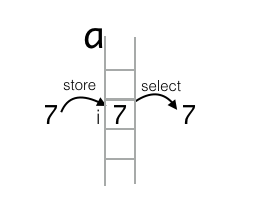
\includegraphics[scale=0.5]{pictures/axiom1.png}

  \end{multicols}
  
\item selecting from a previous store:
  \begin{multicols}{2}
  $$ \forall a i j, i \neq j \to \textsf{select } (\textsf{store } a\ j\ e)\ i = \textsf{select } a i$$
  which means that storing an element has not effect on what can be selected at other indices.

  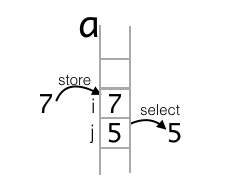
\includegraphics[scale=0.5]{pictures/axiom2.png}
  \end{multicols}
  
\item and extensionality:
  
  \begin{multicols}{2}
  $$ \forall a b, (\forall i, \textsf{select } a\ i = \textsf{select } b\ i) \to a = b$$
  which means that arrays which agrees on elements for every indices can be considered equal.

  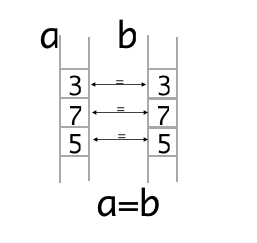
\includegraphics[scale=0.5]{pictures/axiom3.png}
  \end{multicols}
  \end{enumerate}
  

The theory of arrays can be augmented with uninterpreted functions and linear arithmetic (\emph{QF\_AUFLIA}) and to allow a limited form of quantification (\emph{AUFLIA})


\section{Overview of our Solution}

In the remainder of this report, we present our solution which consist of encoding list operations as operation over arrays in various SMT theories. While simple operations such as \lstinline|nth| and \lstinline|upd_nth| can be encoded in the quantifier-free fragment of the theory of array with uninterpreted functions and linear arithmetic \emph{QF\_AUFLIA}, other operations require stronger theories such as \emph{AUFLIA}. 

Targeting \emph{QF\_AUFLIA} is a pragmatic choice. While the theory of inductive datatypes would lead to a direct encoding of lists and list operations, its support is not planned for SMTcoq and would require significant extension to SMTlib and CVC4 (which supports the theory but does not generate proof witness for it). 

%dev
\subsection{A High-Level View of the Envisioned Machinery}
The following graphics describes the different components and the steps that goes into automatically proving an SMT goal using an SMT solver. Doted line represents works done by external tools, where full lines are specific to this project. 

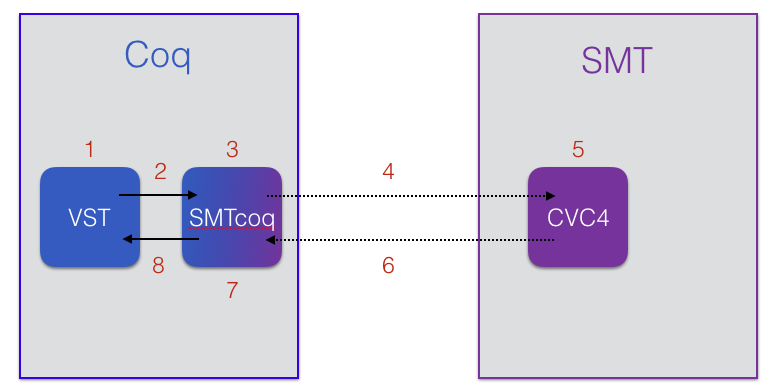
\includegraphics[scale=0.5]{pictures/arch.png}



\begin{enumerate}
\item %1
  A tactic provided by VST isolates the propositional portion of goals from separation-logic predicates.
\item %2
  The propositional goal is encoded into a Coq representation of a datatype which can be manipulated by SMT theories.
  
\item %3
 SMTcoq reifies the encoded goal as an OCaml datatype representing an SMT query equivalent to the encoded goal
  
\item %4
  SMTcoq generates an SMTlib from the OCaml reification of the goal, and send it to CVC4, an SMT solver
  
\item %5
  CVC4 either find a counter example to the query, in which case either the goal is false or it falls into the incomplete portion of the encoding, or it returns UNSAT together with a proof witness of the decision
  
\item %6
  Assuming an UNSAT decision (which asserts the validity of the initial goal), the proof witness is interpreted back in Coq 
  
  
\item %7
  The proof witness is verified by the certified SMT solver included in SMTcoq and the decision is reflected back in Coq as a proof of the encoded goal
  
\item %8
  By soundness of encoding, we use the validity of the encoded goal to prove the validity of the initial goal

  
\end{enumerate}


\subsection{Encoding Lists as Arrays}

% difference between list and QF_AX
In Coq, lists are an inductive datatype representing an ordered collection of finitely many elements of a given type. 
\begin{lstlisting}
inductive list A : Set :=
 | nil : list A
 | cons : A -> list A -> list A.
\end{lstlisting}

In VST, C arrays are reasoned about propositionally as list, using total operation such as \lstinline|upd_Znth| and \lstinline|nthZ|, using mathematical integers as index and a default value as argument to \lstinline|nthZ| returned when accessing the array out of bound. 

As seen in the previous section, the arrays manipulated in \emph{QF\_AX} are associative arrays rather than programmatic ones. They represent an infinite collection of key-value pair where the keys are mathematical integers. 

The basis of our encoding is that the \emph{QF\_AX} array \lstinline|a| representing Coq list \lstinline|l| will be constrained to contain the same elements as \lstinline|l| from indices $0$ to $\mathsf{length} l - 1$ and the default value $d$ otherwise.This means that it should always be the case that
$$ a_i = \textsf{nthZ}\ l\ i\ d$$

Given a goal about lists in VST, we first rewrite it in a three-address code fashion, binding the result of every list operation to a new variable. Then, each operation is encoded according a general, sound correspondence to operations in the theory of arrays:

% encoding of nth
For every goal of the form $s = \textsf{nthZ}\ i\ ls d$, we add the following in the conclusion on the formula sent to the SMT solver:

$$ (0 \leq j < \textsf{len}\ as) \to s = \textsf{select as j}\ \wedge$$
$$\neg (0 \leq j < \textsf{len}\ as) \to s = d $$

Where $as$ is an array corresponding to the list $ls$, and $len$ is an uninterpreted functions which may be constrained by hypothesis in the VST goal about $ls$'s boundaries.


% encoding of upd
$\textsf{upd\_Znth}$ is encoded almost directly by $AX$'s operation $\textsf{store}$. For every goal of the form $s = \textsf{upd\_Znth\ i\ e\ ls}$, we augment the formula with
$$ as' = \textsf{store}\ as\ i\ e \wedge 0 \leq i \leq \textsf{len}\ as \to \textsf{len}\ as' = \textsf{len}\ as$$
which encodes the update operation and the fact that updating within boundaries preserves the length of the list.


% encoding of append
just like $\textsf{nthZ}$, $\textsf{append}$ is encoded using $\textsf{select}$. For every goal of the form $ls = ls_1 ++ ls_2$, we add the following constaints:
$$(0 \leq j < \textsf{len}\ as1) \to \textsf{select}\ as1\ j = \textsf{select}\ as\ j \wedge $$
$$(\textsf{len}\ as1 \leq j < \textsf{len}\ as1 + \textsf{len}\ as2) \to \textsf{select}\ as2\ j = \textsf{select}\ as\ (\textsf{len}\ as1 + j)$$
Under this encoding, the result accessing the resulting array $as$ is equal to the first array $as1$ between $0$ and the length of the first list $ls_1$ and to the second array $as2$ between the length of the first list $ls_1$ and the length of the resulting list $ls$.



\section{Soundness of the Solution, or Reflecting Back on Lists}
% explanation of proof needed for the big picture to work
While we strive for correctness of encoding, differences between lists
and the infinite arrays as manipulated by \emph{QF\_AX} makes such encoding difficult to achieve in general. 
Fortunately, we can instead using a sound, but incomplete encoding, such that the validity 
of the encoding implies the validity of the original formula, but not the other way around.
In other word, some valid goals may result in invalid encodings, but valid encoding only arises from valid goals.

% proof of soundness of encoding
%% QF_AX as Array GDT + Axioms


%% nth as select

%% upd_nth as store

%% ++ as branch-and-select


%end
\section{Future Work}
% 4 pages just there
In the near future, we expect most of the current limitations to our work due to external tools to be lifted.

At the very least, we need CVC4 to generate witnesses for the theory of arrays and SMTcoq to support the theory of arrays and to interface with CVC4. We have the confirmation from the developer of CVC4 and SMTcoq that these are being worked on. In the future, supports for more theories, especially quantified arrays and inductive datatypes, would permit for more direct encodings and, in the case of the latter, automatic generation of encoding together with correctness proof for the datatype and simple functions.

% supporting more list operations and potentially other datatypes
In the meantime, we can extend our encodings with more lists operations, potentially using \emph{AUFLIA} rather than its quantifier-free fragment \emph{QF\_AUFLIA}.

\section{Conclusion}
Our project is meant to be taken as an investigation of the realisability of harnesting an SMT solver to provide automate software verification goals in an interactive theorem prover such as Coq. We conclude that while architecturally we know how to assemble an interface such as this one, the tools which are currently available are too limited for realistic usage.




Even assuming \emph{SMT\_COQ}'s support for CVC4, and CVC4 proof generation for \emph{AUFLIA}, we doubt that our encoding of list goals as array will scale well to more list operations and goals about other inductive datatypes, and that it would be more practical than using the automation facilities already present in Coq. In a more distant future, we envision the support for the theory of inductive datatypes to be of high importance, as it would permit (and potentially generate automatically)  direct encoding of simple Coq datatypes, towards a seamless integration of SMT for VST.


\end{document}
